\documentclass{report}
\usepackage[utf8]{inputenc}
\usepackage{svg}
\usepackage{amsmath}
\usepackage[margin=2cm]{geometry}
\title{CMSC858 Project 1 Report}
\author{Alperen Keles }
\date{March 2022}

\begin{document}

\maketitle

\section*{Introduction}
In this project, I implemented a BitVector implementation, used it for implementing Rank \& Select data structures, which are very useful succint data structures for indexing and querying large amounts of data efficiently. I then implemented an efficient generic Sparse Array using these primitives. 
\section*{Difficulties}
I had a set of problems.
\begin{itemize}
    \item Rust induced problems(no existing good bitvector library, problems migrating from rank/select classes to sparse array because of interface differences).
    \item Abstraction induced problems(Theoretical bounds are great, but they are abstract. Moving down to the code level creates practical challenges on them, so if I were to reimplement this library I wouldn't really stuck with the theoretical bounds, rather move to a more relaxed frame where I still have the asymptotical guarantees ).
\end{itemize}
\section*{Results}
This sections has the results and their short discussions.
\newpage

\subsection*{Rank Structure Generation(Time)}
\subsubsection*{Graph}

\begin{figure}[h!]
    \centering
    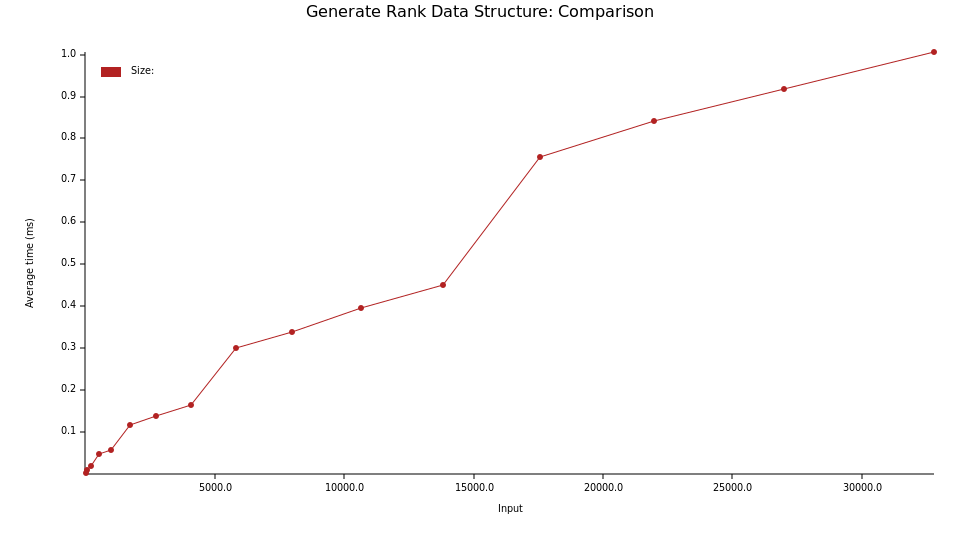
\includegraphics[scale=0.5]{generate_rank_time.png}
    \caption{BitVector Size vs Rank Data Structure Generation Time Graph}
    \label{fig:my_label}
\end{figure}

\subsubsection*{Discussion}
This graphic is linearly growing as expected. Generation of superblock/blocks and lookup tables take linear time with respect to the size of the bitvector. 

\newpage

\subsection*{Rank Structure Generation(Size)}

\subsubsection*{Graph}

\begin{figure}[h!]
    \centering
    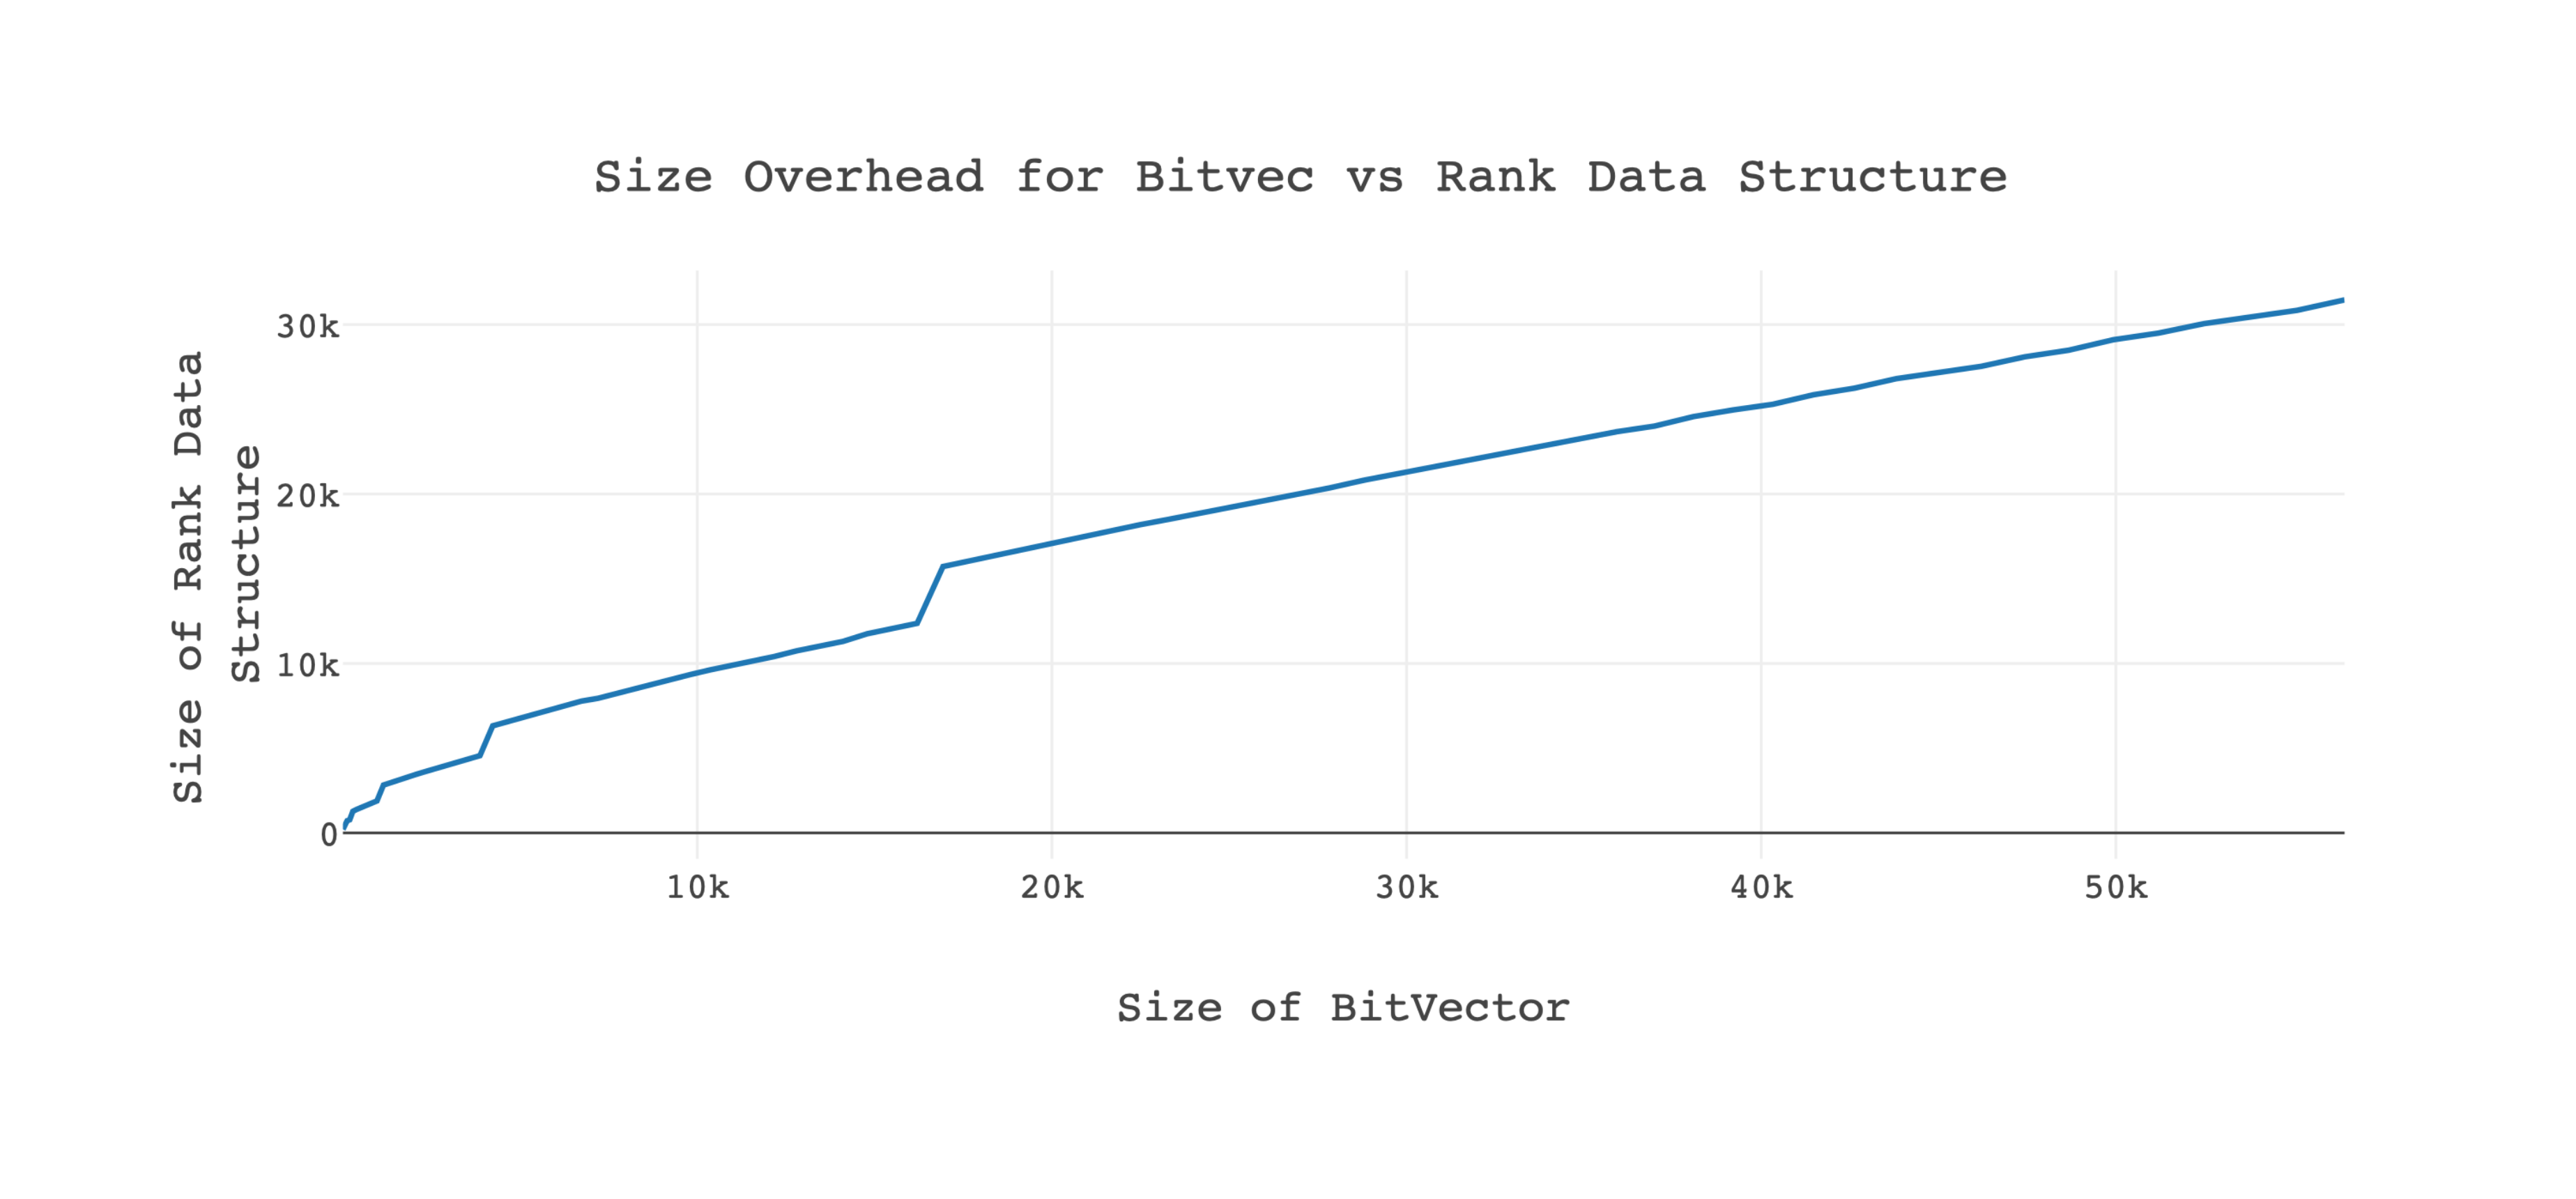
\includegraphics[scale=0.15]{diagram-20220306.png}
    \caption{BitVector Size vs Generated Rank Data Structure Size Graph}
    \label{fig:my_label}
\end{figure}

\subsubsection*{Discussion}
Size of rank data structure follows a $o(N)$ pattern as we theoretically expected. For small values of $N$, fixed overhead might be too much because as opposed to theoretical data structures Rust structs carry metadata, but as we go forward with larger values of $N$, we see structure starts to take less and less space compared to the bitvector size. 
\newpage

\subsection*{Bitvec Size vs Rank1 Time}
\subsubsection*{Graph}
\begin{figure}[h!]
    \centering
    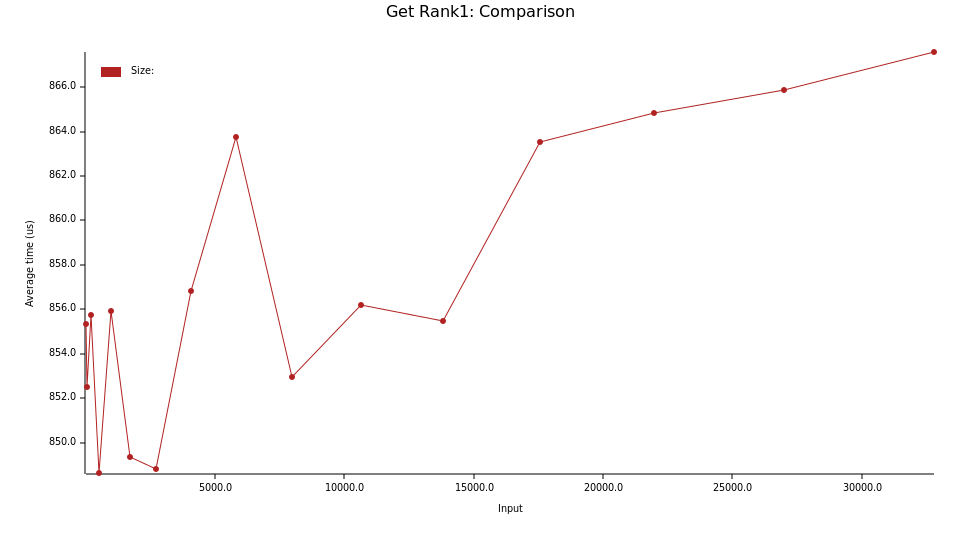
\includegraphics[scale=0.5]{get_rank1_time.png}
    \caption{BitVector Size vs Time for 1000 Rank1 Queries Graph}
    \label{fig:my_label}
\end{figure}
\subsubsection*{Discussion}
This graphic shows our \texttt{rank1} operation is indeed almost constant, is depends very little, and that's due to the implementation of \texttt{BitVector Extraction} function, which if I tried to write efficiently would be out of scope of this homework, and I knew the size would be bounded hence theoretical constant bounds are not broken. 
\newpage

\subsection*{Bitvec Size vs RankN Time}
\subsubsection*{Graph}
\begin{figure}[h!]
    \centering
    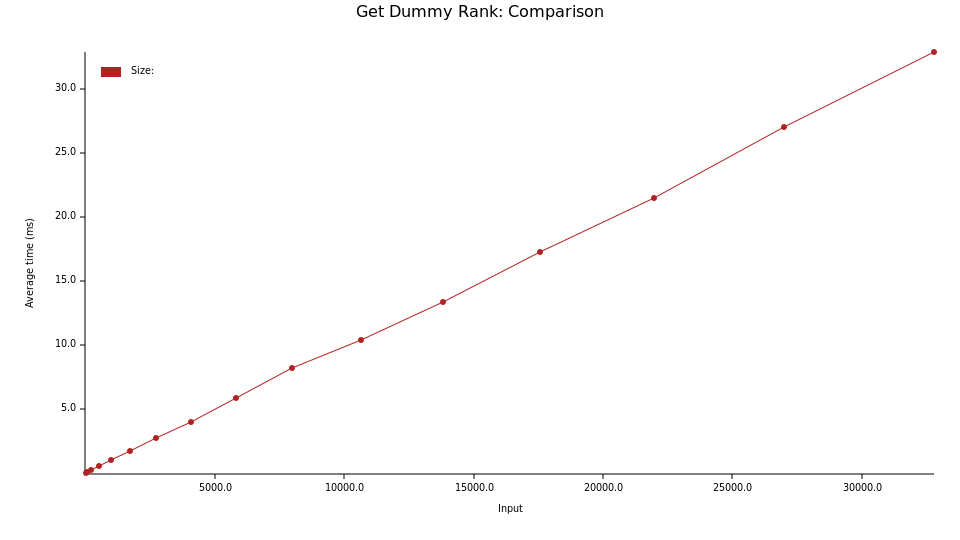
\includegraphics[scale=0.5]{get_dummy_rank_time.png}
    \caption{BitVector Size vs Time for 1000 RankN Queries Graph}
    \label{fig:my_label}
\end{figure}
\subsubsection*{Discussion}
This is the graph of linear time rank operation. It was used as a baseline, ground truth for tests, and also used in the generation of the lookup table. It grows linearly as expected. 
\newpage


\subsection*{Bitvec Size vs Select1 Time}
\subsubsection*{Graph}
\begin{figure}[h!]
    \centering
    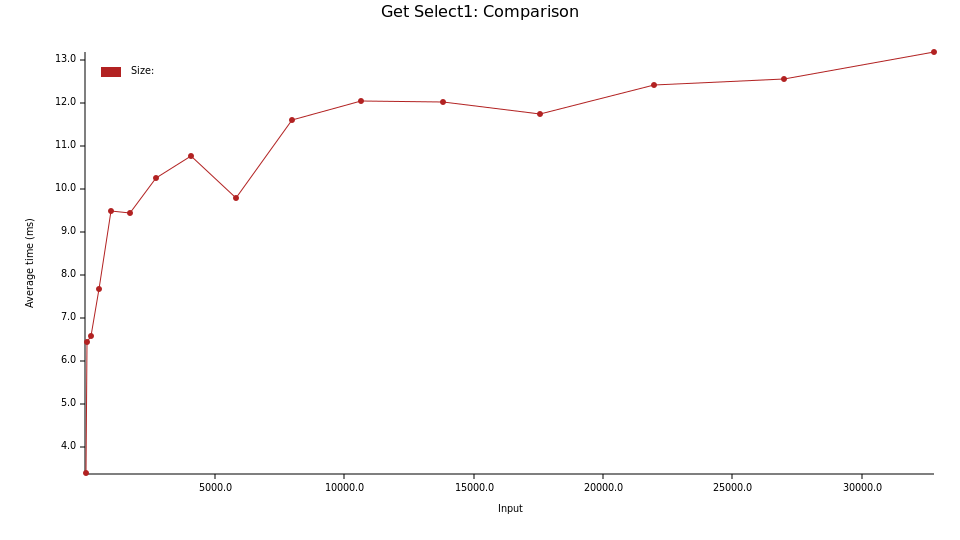
\includegraphics[scale=0.5]{get_select1_time.png}
    \caption{BitVector Size vs Time for 1000 Select1 Queries Graph}
    \label{fig:my_label}
\end{figure}
\subsubsection*{Discussion}
This graphic shows our \texttt{select1} operation is indeed logarithmic. It grows fast at the beginning, yet increase in the time slows down after we reach around 10000 bits. 
\newpage

\subsection*{Sparse Array Generation(Time)}
\subsubsection*{Graph}
\begin{figure}[h!]
    \centering
    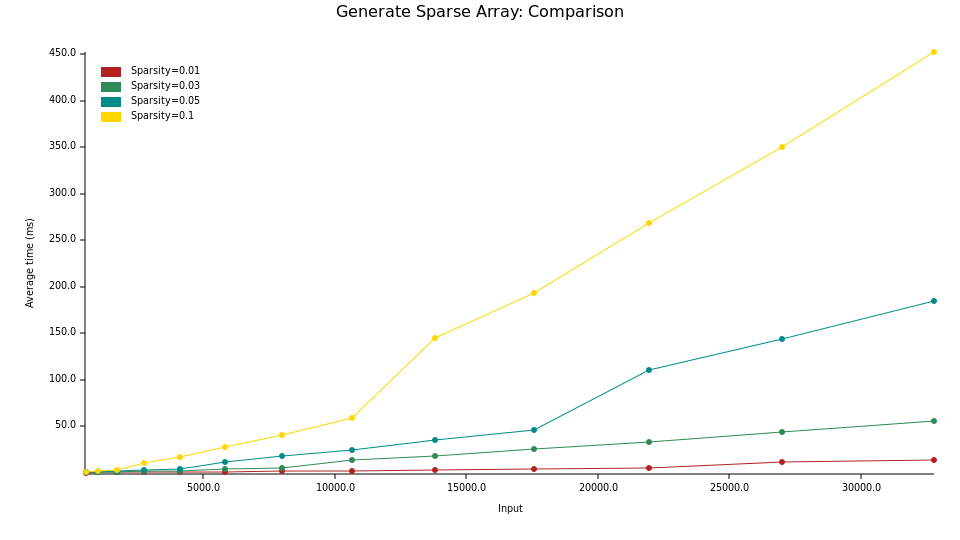
\includegraphics[scale=0.5]{sparse_array_gen_sparsity_vs_size.png}
    \caption{Sparse Array Size/Sparsity vs Time to Generation Graph}
    \label{fig:my_label}
\end{figure}
\subsubsection*{Discussion}
This is the graphic showing how different size/sparsity levels affect generation of a Sparse Array. Affect of size is as expected, linear. Sparsity could be a more surprising result, but this is due to dynamic nature of sparse arrays. Each append operation requires the index to be computed again, which means it takes more time to build the index simply when we do it more times. 
\newpage


\subsection*{Sparse Array Generation(Size)[Theoretical Discussion/Not Implemented]}
This is very much implementation dependent, so I will first lay out my assumptions. \\
-- Naive implementation will use a null pointer based schema rather than a tagged union for empty spaces, as the second one takes much more space, this still fits to our purposes. \\
-- A pointer takes 64 bits/8 bytes space. \\
Then comes our conclusions. \\
1. One can easily see that both implementations take the same space for present elements, as they naively store them. Our bitvector based implementation will probably be better as it holds a continous vector rather than separate elements reached via pointers due to spacial locality. \\
2. Then, we are left with comparing the size of pointer array$(64*size)$ vs the bitvector(size) bits plus the rank data structure($o(size$)). Which means our implementation is at worst 32 times memory efficient, depending on the $o(size)$ factor. \\


\newpage

\subsection*{Sparse Array Rank(Time)}
\subsubsection*{Graph}
\begin{figure}[h!]
    \centering
    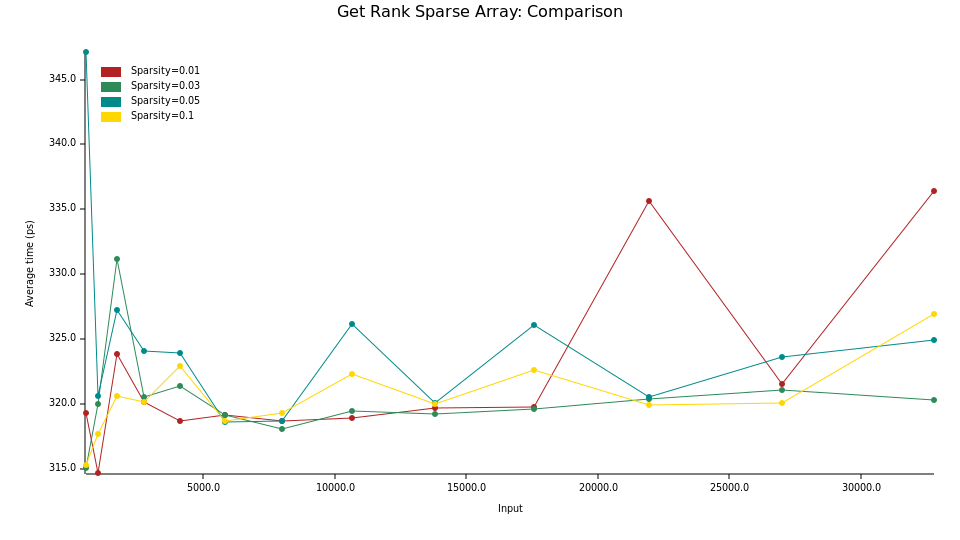
\includegraphics[scale=0.5]{get_rank_size_vs_sparsity.png}
    \caption{Sparse Array Size/Sparsity vs Time for 1000 Rank Queries Graph}
    \label{fig:my_label}
\end{figure}
\subsubsection*{Discussion}
For this function, I rely on random access over the vector. Hence, it's so low(on the order of picoseconds) on time. I believe the fluctuations are due to me using my computer, while holding the experiments. 
\newpage

\subsection*{Sparse Array Index(Time)}
\subsubsection*{Graphic}
\begin{figure}[h!]
    \centering
    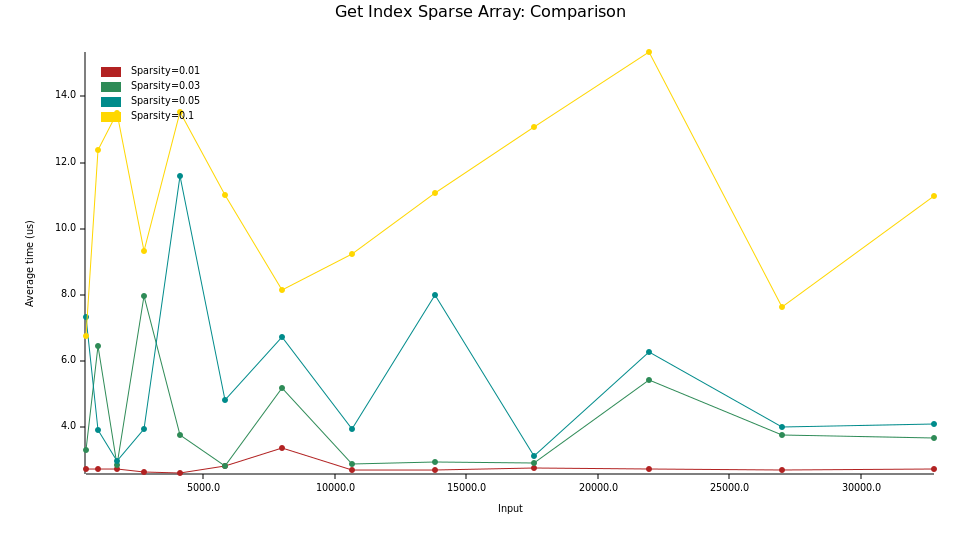
\includegraphics[scale=0.5]{get_index_size_sparsity.png}
    \caption{Caption}
    \caption{Sparse Array Size/Sparsity vs Time for 1000 Index Queries Graph}
\end{figure}
\subsubsection*{\subsubsection*{Discussion}}
For this function, I rely on the rank function of \texttt{rank\_support} structure. I believe that the fluctuations are again to due me using my computer while holding the experiments and also the order being very low again(microseconds) so it's easily disturbed. Yet, we see a significant impact from sparsity, this is due to empty accesses. For empty position accesses, we don't need to do any query, which as I mentioned very close to constant yet not really constant due to \texttt{extract} function. 
\newpage


\end{document}
